%!TEX TS-program = xelatex
%!TEX root = ../../maxwell2018thesis.tex

\chapter[A Background of Stopping in IIR]{A Background of Stopping in\\Interactive Information Retrieval}\label{chap:stopping_background}

\section{Measures}

\section{Stopping Heuristics}

\section{User Studies}

\section{Models of Search}

\subsection{Conceptual Models}
The Berry Picking Model

\begin{figure}[t!]
    \centering
    \resizebox{1\hsize}{!}{
    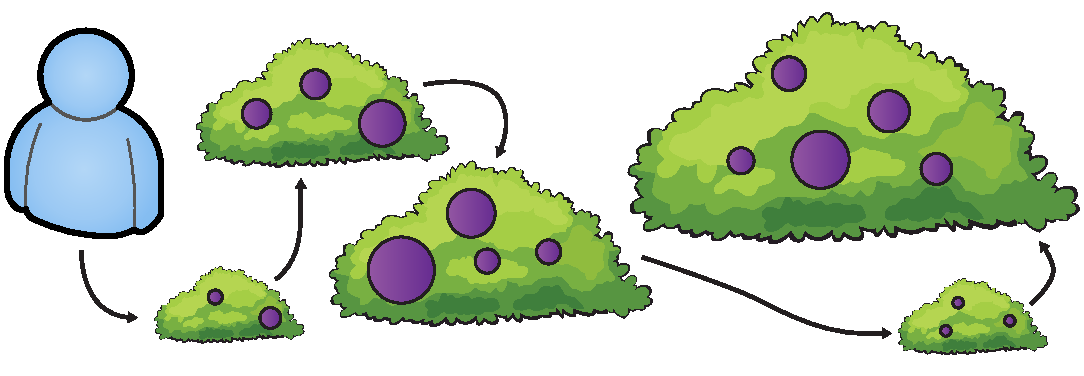
\includegraphics{figures/ch3-berry_picking.pdf}}
    \caption[The Berry Picking Model~\cite{bates1989berry_picking}]{The Berry Picking Model, defined by~\citealt{bates1989berry_picking}.}
    \label{fig:baskaya_model}
\end{figure}


\subsection{Information Foraging Theory}

\subsection{(Interactive) Probability Ranking Principle}

\subsection{Search Economic Theory}

\subsection{Paul Thomas Model}

\subsection{Feza Model}

\begin{figure}[t!]
    \centering
    \resizebox{1\hsize}{!}{
    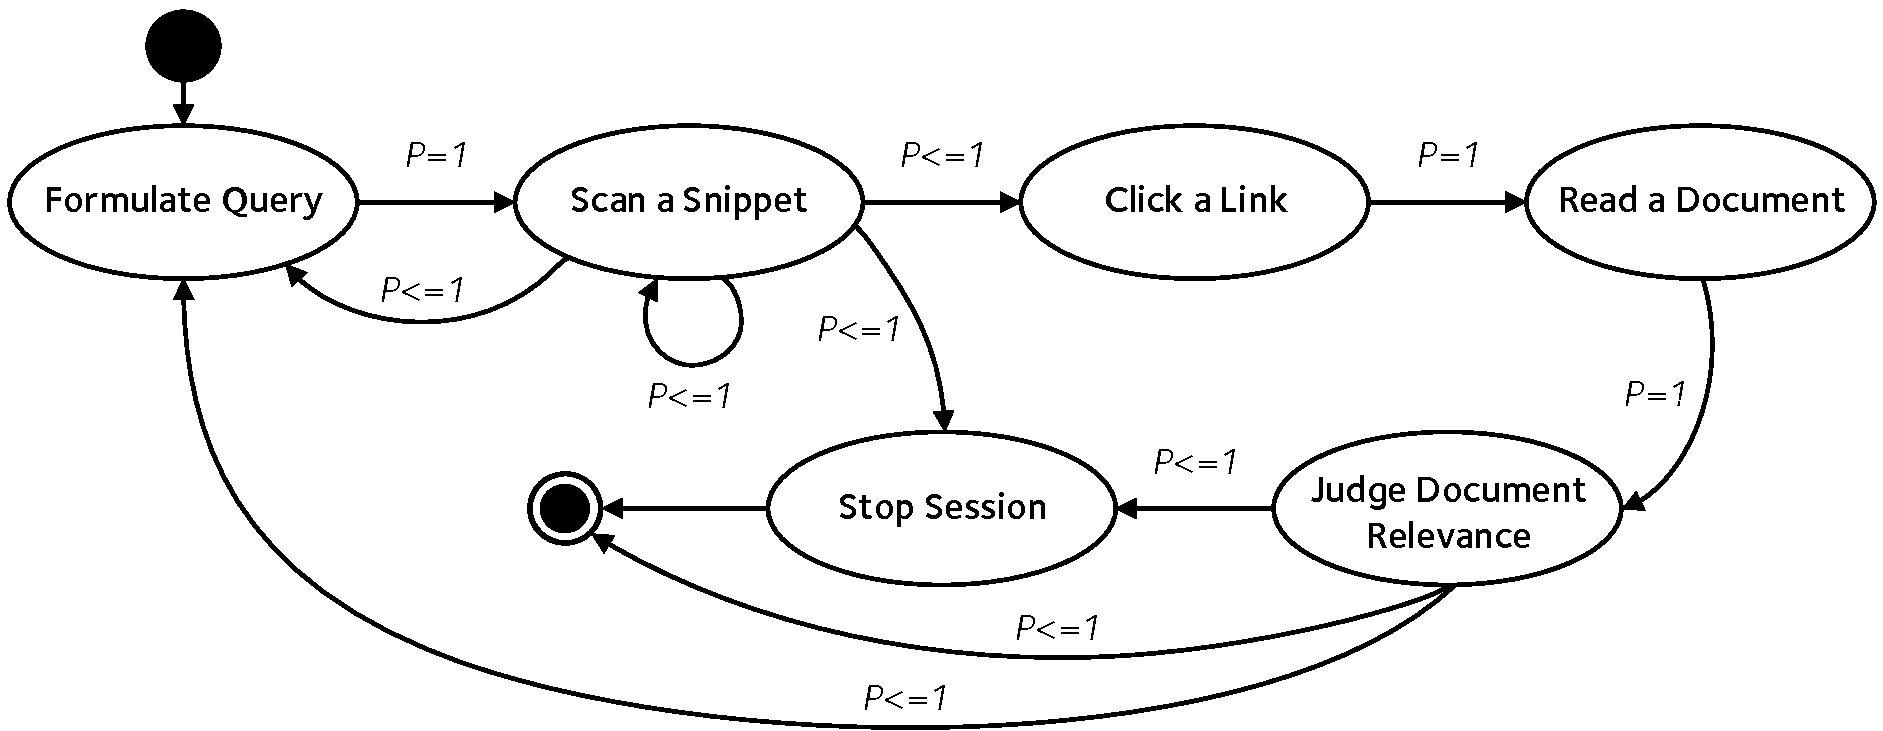
\includegraphics{figures/ch3-baskaya.pdf}}
    \caption[Model of the search process by~\cite{baskaya2013behavioural_factors}]{The user model of search, as outlined by~\citealt{baskaya2013behavioural_factors}. Represented as a Markov Model, the model considers six steps in all. Encoded within two of the steps are decision points that a user following this model must consider in order to continue. Figure adapted (with permission) from the authors of~\citealt{baskaya2013behavioural_factors}.}
    \label{fig:baskaya_model}
\end{figure}

\begin{figure}[t!]
    \centering
    \resizebox{1\hsize}{!}{
    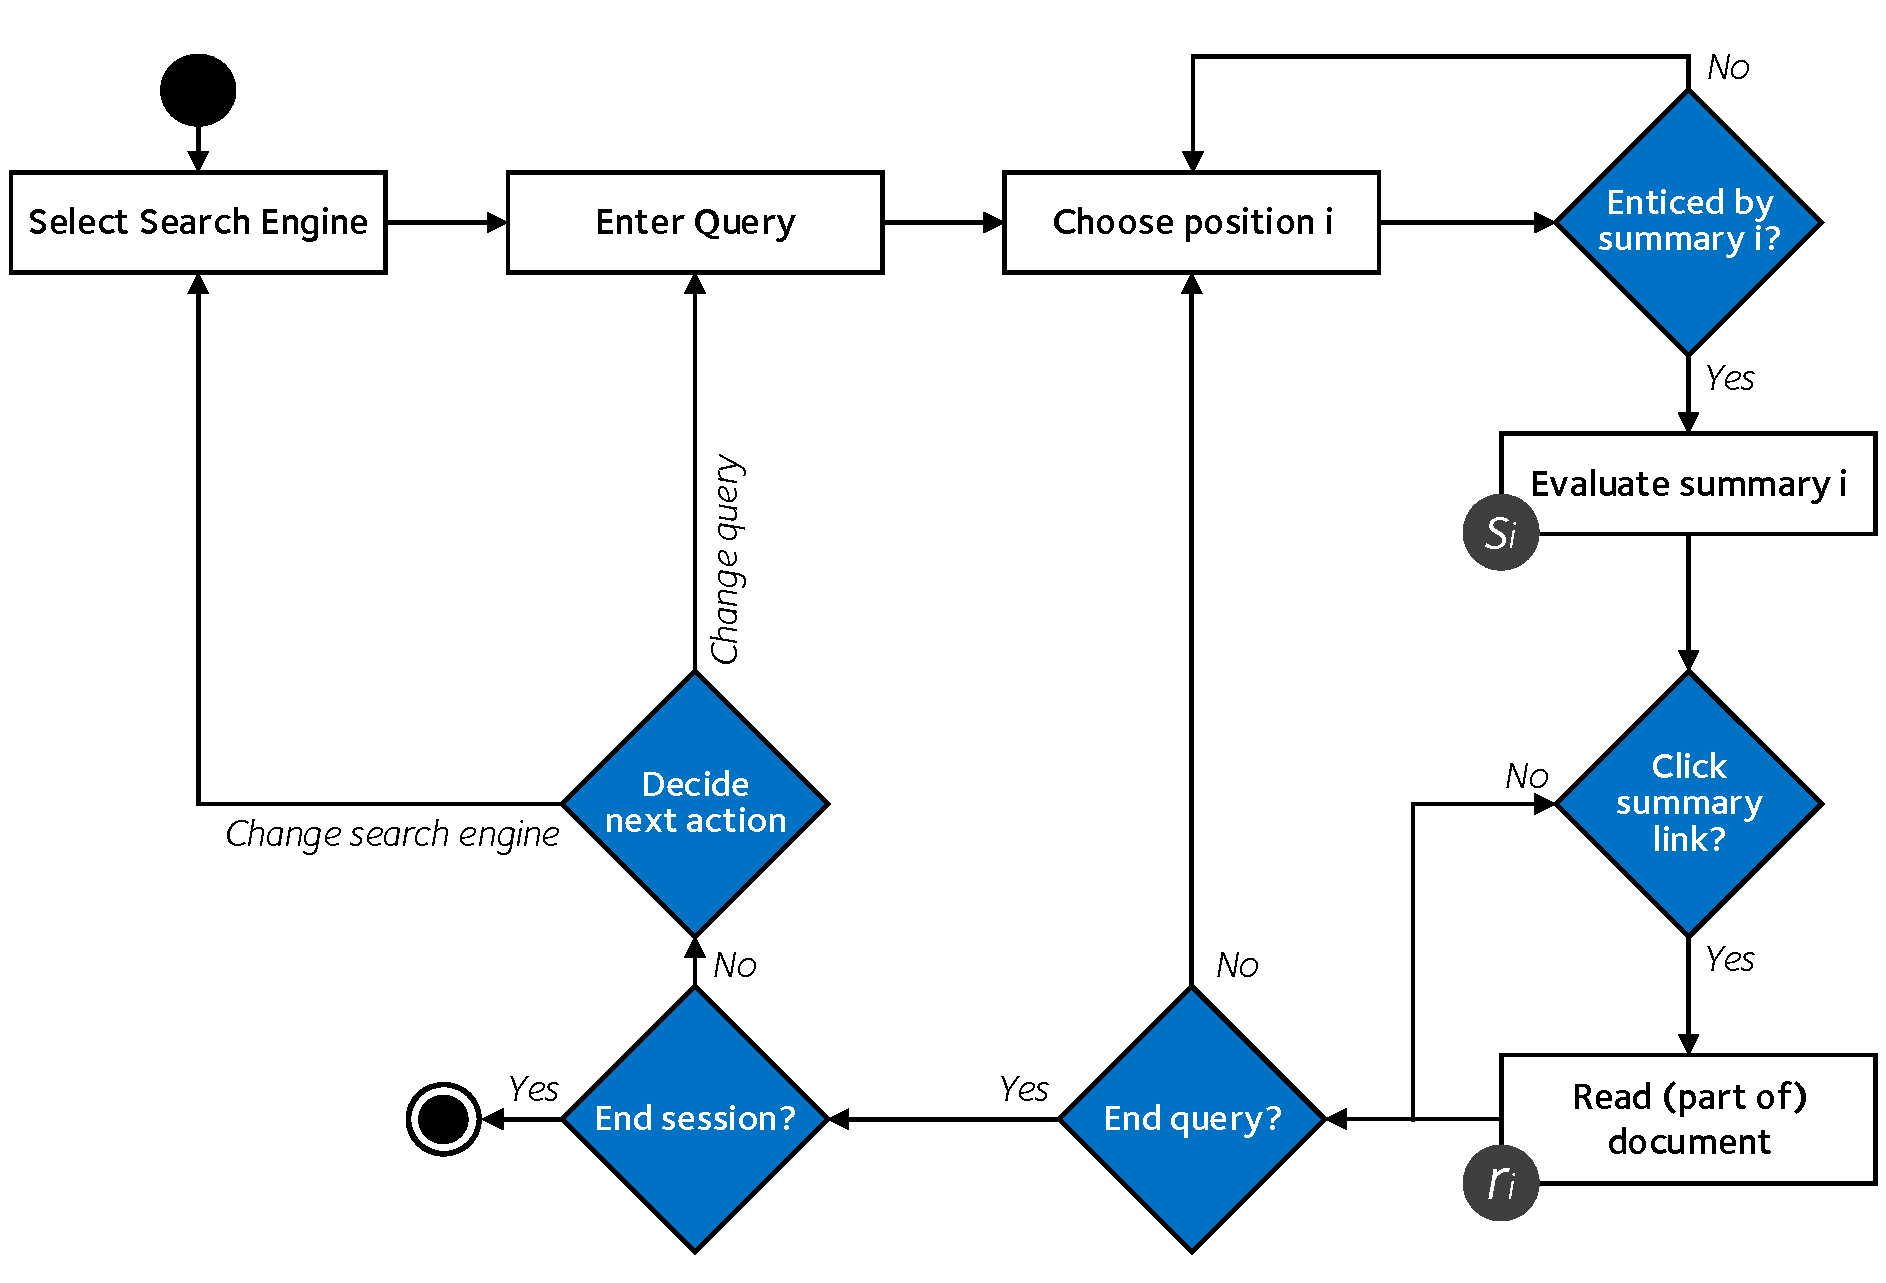
\includegraphics{figures/ch3-thomas.pdf}}
    \caption[Model of the search process by~\cite{thomas2014modelling_behaviour}]{A model of the search process, considering the high-level processes undertaken by a searcher, as outlined by~\cite{thomas2014modelling_behaviour}. Also included are a number of decision points (represented as diamonds) that searchers must consider when following this model. Figure adapted (with permission) from the authors of~\citealt{thomas2014modelling_behaviour}. \textcopyright~Paul Thomas, Peter Bailey, Alistair Moffat and Falk Scholer.}
    \label{fig:thomas_model}
\end{figure}


Refer to the following chapter for more information on how we extend these models to make them more realistic.

\section{Chapter Summary}